\include{template}
%\cfoot{} %% if no page number is needed

\begin{document}

\begin{header}
Activité 2 -- Identification d'espèces
\end{header}

\section*{Test caractéristique du}

\begin{figure}[h]
\center
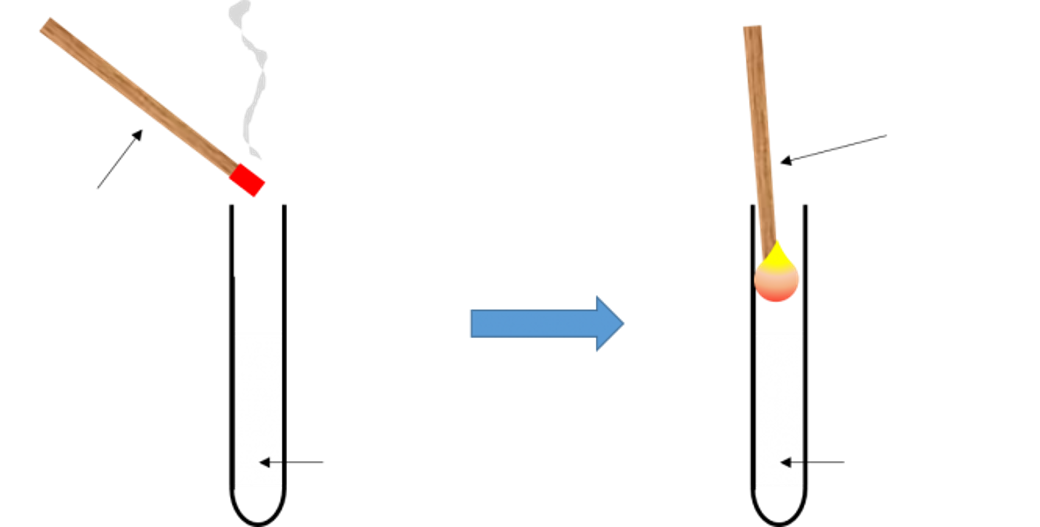
\includegraphics[height=140pt]{images/test_o2.png}
\end{figure}

\section*{Test caractéristique du}

\begin{figure}[h]
\center
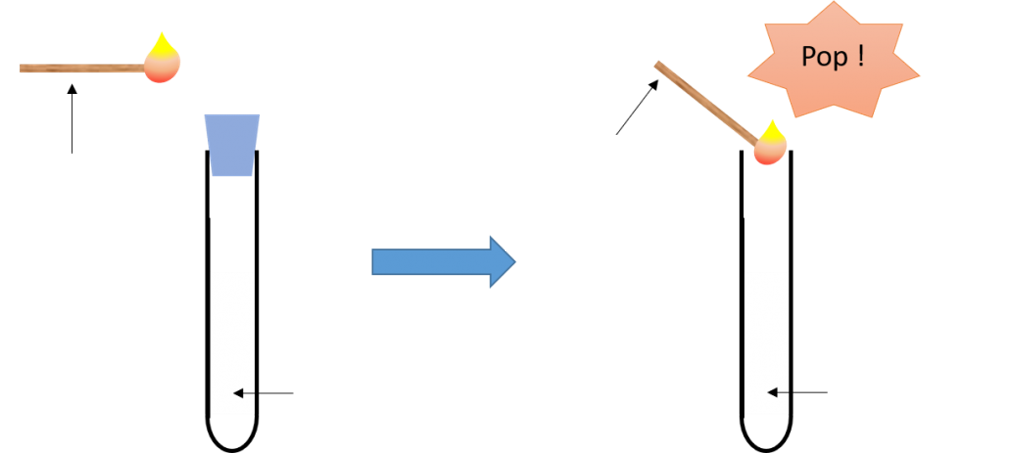
\includegraphics[height=140pt]{images/test_h2.png}
\end{figure}

\section*{Test caractéristique du}

\begin{figure}[h]
\center
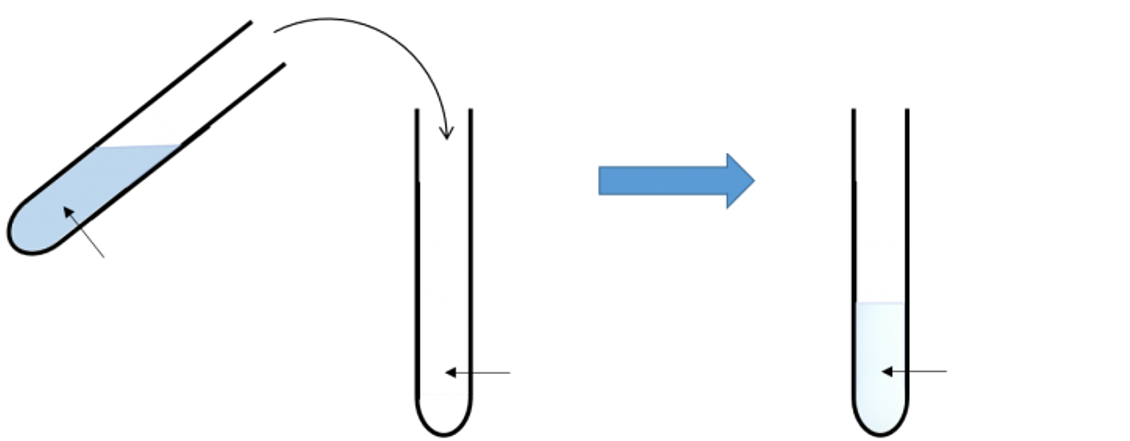
\includegraphics[height=130pt]{images/test_co2.png}
\end{figure}

\begin{enumerate}
\item Compléter les schémas des tests caractéristiques utilisés pour identifier quelques gaz et donner le nom du gaz mis en évidence.
\end{enumerate}

\newpage

\begin{table}[h]
\center
\begin{tabular}{l|c|c|c|c|c|c|c}
Substance & Eau & Glycérol & Ethanol & Kérosène & Cyclohexène & Butan-2-ol & Diazote \\
\hline
\hline
$\rho$ ($\mathrm{kg/L}$) & & 1{,}26 & 0{,}79 & 0{,}80 & 0{,}81 & 0{,}81 & 0{,}81 \\
$d$ & & & & & & \\
$T_\mathrm{fus}$ ($\degree\mathrm{C}$) & & 18{,}2 & -114 & -48 à -26 & -104 & -115 & -210 \\
$T_\mathrm{eb}$ ($\degree\mathrm{C}$) & & 290 & 78{,}4 & 150 à 300 & 83{,}3 & 99{,}5 & -196 \\
$n$ & 1{,}330 & 1{,}473 & 1{,}359 & 1{,}448 & 1{,}445 & 1{,}393 & 1{,}0003
\end{tabular}
\caption{Propriétés physiques de quelques substances : masse volumique $\rho$ (au point d'ébullition), densité $d$, température de fusion $T_\mathrm{fus}$, température d'ébullition $T_\mathrm{eb}$ et indice de réfraction $n$ (à $\unit{25}{\celsius}$).}
\end{table}

\begin{enumerate}
\setcounter{enumi}{1}
\item Compléter la colonne sur les propriétés de l'eau : $\rho$, $T_\mathrm{fus}$, $T_\mathrm{eb}$.
\end{enumerate}

\section*{Masse volumique}

\begin{enumerate}
\setcounter{enumi}{2}
\item Est-il possible d'identifier les différentes substances en mesurant leur masse volumique ?
Justifiez votre réponse.
\item Rappeler la définition de la densité $d$ d'un liquide. Quelle est son unité ? Compléter la ligne correspondante du tableau.
\end{enumerate}

\section*{Changements d'état : \href{https://tinyurl.com/yxmtwo32}{https://tinyurl.com/yxmtwo32}}

\begin{enumerate}
\setcounter{enumi}{4}
\item Sous quelle forme trouve-t-on les différentes substances du tableau à \unit{15}{\celsius} ?
\item Rappeler le nom des différents changements d'état qui existent entre solide, liquide et gaz.
\item En observant les températures de changement d'état, identifier le\cdot s mélange\cdot s.
\end{enumerate}

\section*{Chromatographie : \href{https://tinyurl.com/y6neowtg}{https://tinyurl.com/y6neowtg}}

\begin{figure}[h!]
\center
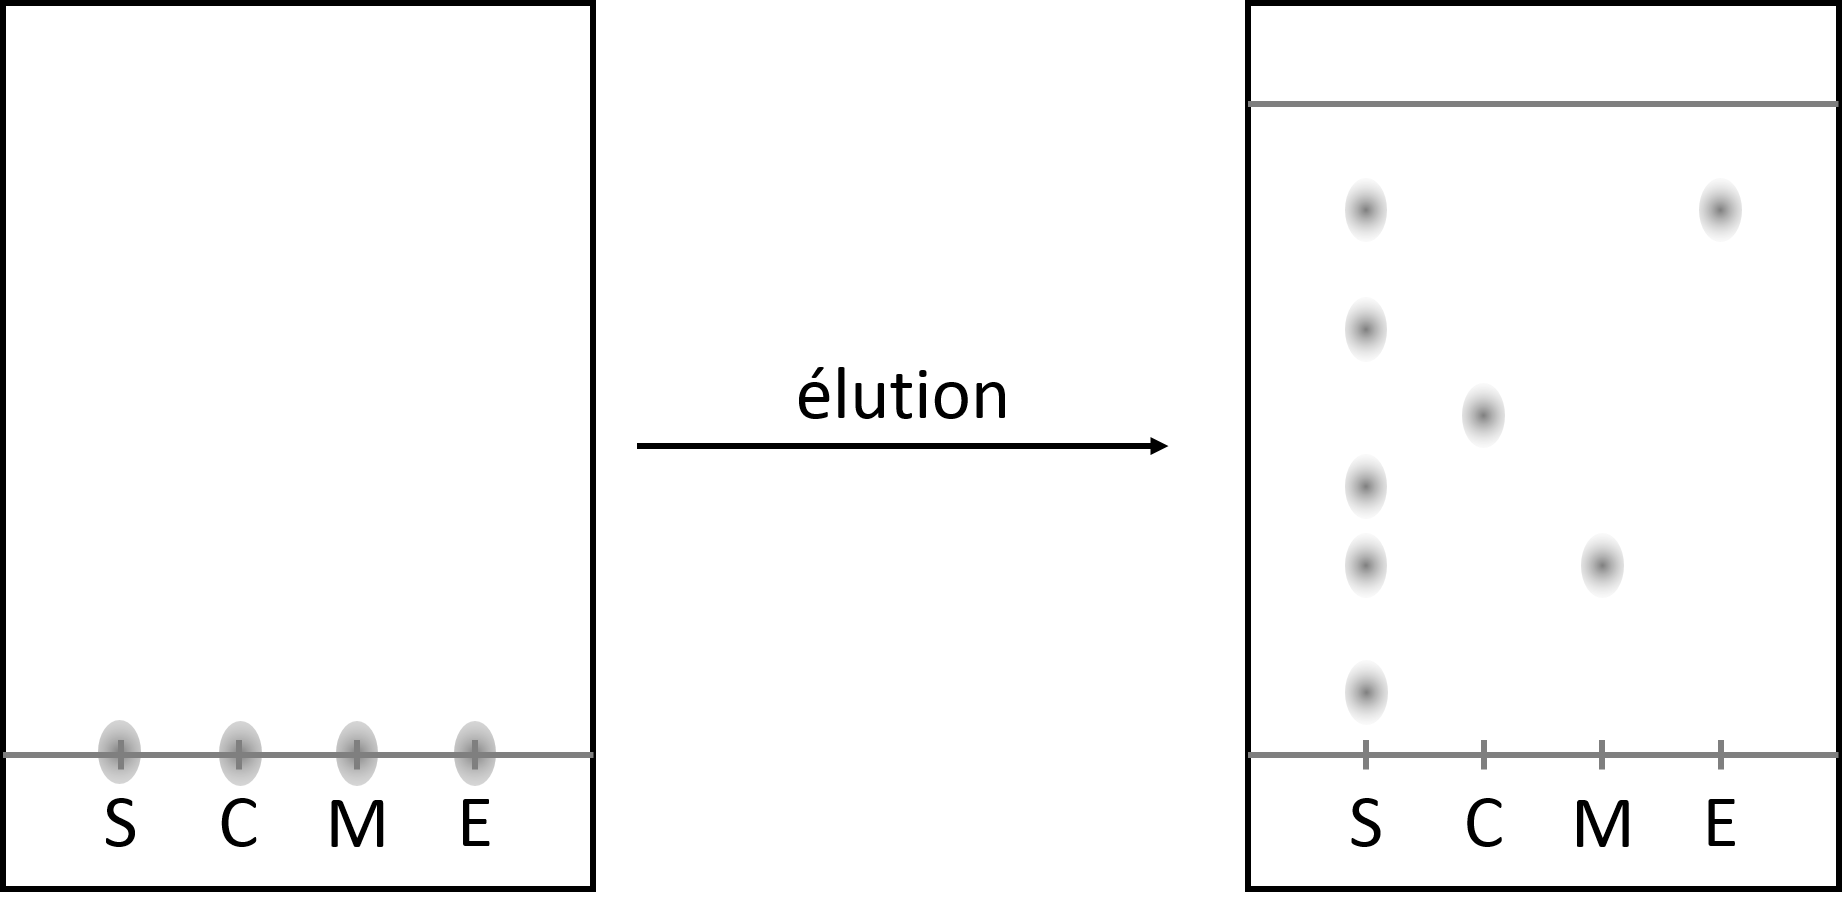
\includegraphics[scale=0.25]{images/ccm.png}
\end{figure}

On souhaite analyser la composition d'une pastille utilisée pour rafraichir l'haleine.
Pour cela on réalise une chromatographie sur couche mince (CCM) : sur la ligne de dépôt on dépose en S une goutte de solution préparée à partir de la pastille, en C du citral, en M du menthol et en E de l'eucalyptol.

\begin{enumerate}
\setcounter{enumi}{7}
\item Faire un schéma du montage expérimental utilisé pour réaliser l'élution.
\item Sachant que les espèces analysées sont toutes incolores, comment révéler le chromatogramme ?
\item Nommer les espèces chimiques identifiables entrant dans la composition de la pastille.
\end{enumerate}

\end{document}